% -*- TeX -*- -*- DE -*-

\chapter{Grundlagen}\label{ch:Grundlagen}
Hier wird kurz aufgezählt was erläutert wird. Mehr nicht. \
Es sollen hier nur Elemente erläutert werden, die für mindestens zwei der Methoden relevant sind.\
k-center greedy (PatchCore), Autoencoder (efficientad) oder Backpropagation (simplenet) also zB nicht.\

\section{Datensatz: MVTecAD}\label{sec:DatensatzMVTecAD}
Erläuterung des Datensatzes MVTecAD. Beispielbilder.

\section{Eigener Datensatz (Granulat)}\label{sec:EigenerDatensatz}
Details und Beispiele zu eigenem Datensatz.

\section{Residuale Netzwerke}\label{sec:ResidualNetworks}
In diesem Abschnitt werden die Grundlagen von Residual Networks (textbf{\glqq ResNets\grqq{}}) erläutert. \
Diese spielen für die Merkmalsextraktoren (\glqq Feature Extractors\grqq{}) in den im Haupteil der Arbeit (TODO --> Link) eine wichtige Rolle. \
Der Schwerpunkt hierbei liegt auf der grundlegenden Idee, der Rolle, die ResNets historisch in der Entwicklung von Deep Learning gespielt haben und \
vor allem den Aspekten, die für die Anwendung in dieser Arbeit relevant sind. \ 
Für detailierte Informationen zu ResNets wird auf das Paper von Kaiming He et al. \cite{resnet} und die zahlreichen Erläuterungen in der Literatur verwiesen. \
\subsection{Hintergrund \& Idee hinter \glqq ResNets\grqq{}}\label{subsec:ResNetsBackgroundAndIdea}
%Deep Neural Networks (DNNs) are excellent at learning hierarchical representations from data, but they face challenges as they become deeper. One of the primary issues is the vanishing gradient problem, where gradients during training become extremely small as they are backpropagated through many layers. This makes it challenging to update the weights of early layers, hindering the learning process.
Tiefe neuronale Netze (Deep Neural Networks, DNNs) eignen sich hervorragend für das Lernen hierarchischer Darstellungen aus Daten,\
aber sie stehen vor Herausforderungen, wenn sie \glqq tiefer\grqq{} werden.\glqq Tiefe\grqq{} bezeichnet in diesem Zusammenhang \ 
die Anzahl an Schichten, die sequentiell durchlaufen werden, um das Endergebnis bzw. die Ausgabe zu erhalten. \
Tiefere Netze können komplexere Merkmale in Daten erfassen, was für Aufgaben wie die Bildklassifizierung, bei der Objekte und Muster komplizierte Details aufweisen können, entscheidend ist.\
Einer der großen Herausforderungen bei tiefen Netzen ist das Problem der \glqq verschwindenden Gradienten\grqq{} (\textit{engl.} \textbf{Vanishing Gradients}). \
Diese Gradienten sind entscheidend für das Training eines Neuronalen Netzes, insofern, als dass das Optimierungsverfahren des Gradientenabstiegs die Grundlage auch moderner Optimierer wie \glqq Adam\grqq{} (TODO --> Ref) ist. \ 
Dieses Problem lässt sich anschaulich dadurch erklären, dass frühe Gradienten, was sich leicht mithilfe der Kettenregel zeigen lässt, \ 
eine Multiplikation von allen nachfolgenden (im Sinne der Infernenzrichtung - \glqq forward pass\grqq{}) Gradienten darstellt. \
Betrachtet man nun ein sehr tiefes Netz, das heißt, viele Gradienten, die miteinander multipliziert werden und den wahrscheinliche Fall von Gradienten, die kleiner als $1$ sind, so wird schnell klar, dass frühe Schichten einen sehr kleinen Gradienten haben können. \
Dies macht es schwierig, die Gewichte der frühen Schichten zu aktualisieren, was den Lernprozess behindert. Dabei ist es vor allem die Tiefe, die Neuronalen Netzen das Generalisieren von komplexen Zusammenhängen ermöglicht (\glqq Deep Learning \grqq{})\\
Residuale Netze, allgemein bekannt als ResNets und im Folgenden auch so bezeichnet, wurden von Kaiming He et al. (TODO --> Ref) in ihrem Paper von 2015 vorgestellt und bieten eine einfache und dennoch effektive Methode an, wie dieses Problem angegangen werden kann. \
Die Grundidee besteht darin, Verknüpfungen zwischen den Schichten einzuführen, die es dem Netz ermöglichen, eine oder mehrere Schichten zu \glqq überspringen\grqq{}. \ 
Anstatt die gewünschte Abbildung also direkt zu lernen, lernen ResNets die residuale Abbildung, was der Differenz zwischen Ein- und Ausgabe entspricht. Die Eingabe wird über sogenannte \
\glqq Shortcut (Skip) Connections\grqq{}, also einfach die Identitätsabbildung, vom Eingang zur residualen Ausgabe weitergeleitet, um dann durch Summation wieder miteinander verknüpft zu werden. \
Das Problem der verschwindenden Gradienten wird dadurch entschärft, dass die Gradienten direkt in frühere Schichten zurückfließen können. 
Anschaulich lässt sich das durch die Tatsache erklären, dass die Identitätsabbildung einen konstanten Gradienten von $1$ besitzt. Weil sich die Summenbildung \
am Ausgang eines nachfolgend noch im Detail besprochenen Residual-Blocks auch bei der Gradientenbildung als Summation widerspiegelt, ist der Gradient einer jeden Schicht nicht mehr das Produkt, sondern vielmehr die Summe aller nachfolgenden Gradienten. (Optional TODO: Formel) 
Das zugrundeliegende Paper ist eines der meistzitierten Paper im Bereich des Deep Learning und hat die Entwicklung von Deep Learning maßgeblich beeinflusst. \
\subsection{Residual Block \& Architektur}\label{subsec:ResidualBlocks}
%The basic building block of a ResNet is the residual block. It consists of two main paths: the identity path (the shortcut connection) and the residual path (the main convolutional path). Mathematically, the output of a residual block is calculated as:
Der Grundbaustein eines ResNet ist der Residualblock. Er besteht aus zwei Hauptpfaden: dem Identitätspfad (der Abkürzungsverbindung) und dem Residualpfad (dem Hauptfaltungspfad).\ 
Mathematisch wird die Ausgabe eines Residualblocks wie folgt berechnet:
\[
\text{Output} = F(\text{Input}) + \text{Input}
\]
wo $F$ die Residualabbildung ist, die durch die Hauptfaltungsschichten gelernt wird.\  
%The shortcut connection allows the gradients to flow directly back to earlier layers without vanishing, making it easier for the network to learn.
Nachfolgende Abbildung zeigt eine vereinfachte Darstellung eines \glqq Building Blocks\grqq{} bzw. Residual Block. \
\begin{figure}[H]
  \centering
  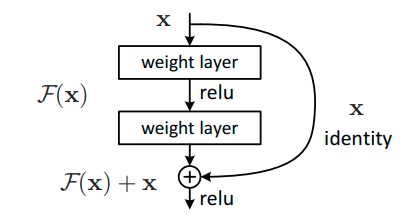
\includegraphics[width=0.5\textwidth]{bilder/residual_block.png}
  \caption{Residual Block (TODO --> Ref)}
  \label{fig:ResidualBlock}
\end{figure}
Ein ResNet besteht aus mehreren Residualblöcken, die sequentiell durchlaufen werden. Es ist also eine \glqq Feed-Forward\grqq{}-Architektur, weil die Daten zur Inferenz \ 
nur in eine Richtung durch das Netz fließen. Durch das \glqq Stapeln \grqq{} können dann sehr tiefe Netze erstellt werden, die sich dennoch aufgrund der oben beschriebenen
Eigenschaften gut optimieren bzw. trainieren lassen. \\
Es existieren zahlreiche verschiedene Varianten von ResNets, die sich in der Art und Anzahl ihrer Residual Blöcke unterscheiden. \
Nachfolgende Tabelle gibt einen Überblick über die drei, in dieser Arbeit vor allem verwendeten Varianten: ResNet18, ResNet34 und WideResNet50 \

\begin{table}[h]
  \centering
  \begin{tabular}{|c|c|c|c|c|}
  \hline
  \textbf{Netzwerk} & \textbf{Tiefe} & \textbf{\# Parameter} & \textbf{Top-1 Fehlerrate\tablefootnote{in ILSVRC (TODO --> Ref)}} & \textbf{Inferenz auf RBP4\tablefootnote{Raspberry Pi 4B 8GB. Betrachtet wurde die Laufzeit von einem Bild der Auflösung 224x224 und 3 (Farb-)Kanälen}} \\ \hline
  ResNet18         & \makecell{$18$}             & \makecell{$\num{11,7e6}$}                        & \makecell{$\num{30.24}$\%}                   & \makecell{$0,82\si{\second}$}\\ \hline
  ResNet34         & \makecell{$34$}             & \makecell{$\num{21,8e6}$}                       & \makecell{$\num{26.70}$\%}                   & \makecell{$1,45\si{\second}$}\\ \hline
  WideResNet50     & \makecell{$50$}             & \makecell{$\num{68,9e6}$}                        & \makecell{$\num{22.53}$\%}                   & \makecell{$3,00\si{\second}$}\\ \hline
  \end{tabular}
  \caption{Vergleich verschiedener ResNet Varianten (TODO --> Ref)}
  \label{tab:resnet-comparison}
\end{table}
Zu erkennen ist eindeutig, dass die Anzahl der Parameter und die Inferenzzeit mit der Tiefe des Netzes steigt. \
Gleichzeitig lässt sich aber auch eine Verbesserung der Top-1 Fehlerrate erkennen, je tiefer bzw. mächtiger das Netz ist. \\
Einer der Hauptvorteile von ResNets ist die Fähigkeit, Merkmale pyramidenförmig durch das Netz zu verbreiten. Das bedeutet, dass das Netz Merkmale auf verschiedenen \ 
Abstraktionsebenen erfassen kann, von Low-Level-Merkmalen wie Kanten und Ecken bis zu High-Level-Merkmalen wie Objektteilen und semantischen Konzepten. \
Mit zunehmender Tiefe wird also die Auflösung der \glqq Feature Maps\grqq{} (TODO --> Ref) reduziert, während die Anzahl der Kanäle und die Komplexität der zugrundeliegenden Merkmale zunimmt. \
Dargestellt ist das in folgender Abbildung:
\begin{figure}[H]
  \centering
  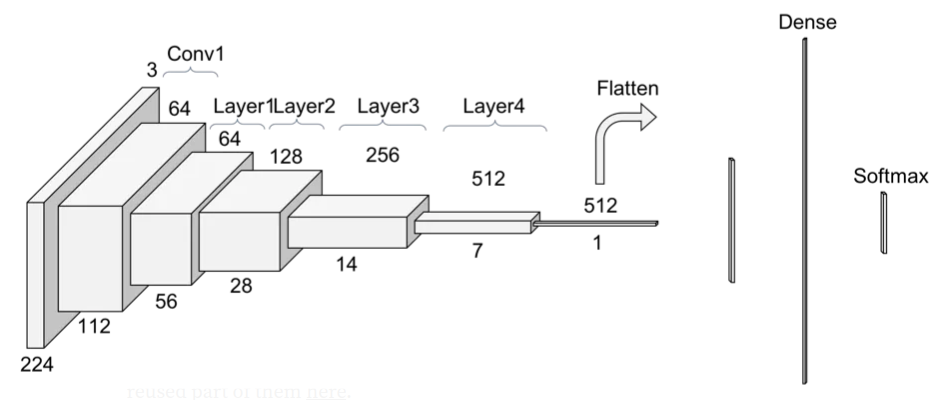
\includegraphics[width=0.8\textwidth]{bilder/resnet_pyramid.png}
  \caption{Pyramidale Merkmalsverteilung in ResNets (TODO --> Ref)}
  \label{fig:ResNetPyramid}
\end{figure}

Die Quader in oben stehendem Netz stehen symbolhaft für die Auflösung der Feature Maps. \
Während die oben stehenden Zahlen die Anzahl der Kanäle repräsentieren, stehen die unten aufgeführten Zahlen für die räumliche Auflösung. Letztere hängt \ 
proportional von der Auflösung des Eingangsbildes ab und gilt für alle drei Modelle. Die Anzahl an Kanälen ist konstant für alle Auflösungen und für ResNet18 und ResNet34. \
Für das WideResNet50 gilt im Wensentlichen der gleiche Aufbau, allerdings sind die Kanäle \glqq geweit\grqq{} gegenüber den anderen beiden Architekturen, was \
sich an der Vervierfachung der Anzahl an Kanäle durch Verwendung eines komplexeren Residual Blocks (\glqq Bottleneck\grqq{}\cite{wideresnet})zeigt. 
ResNet18 und ResNet34 unterscheiden sich ausschließlich in der Anzahl der Residual Blöcke bzw. der Tiefe des Netzes. \\
Alle der drei hier vorgestellten Architekturen lassen sich in fünf Faltungsschichten (\glqq Conv1\grqq{}, \glqq Layer1\grqq{}, \glqq Layer2\grqq{}, \glqq Layer3\grqq{}, \glqq Layer4\grqq{}) unterteilen. \
Dem schließt sich eine \glqq Average Pooling\grqq{}-Schicht an, die die Auflösung der Feature Maps auf 1 reduizert (\glqq Flatten\grqq{}). Dieser 1D-Vektor wird \
schließlich durch eine \glqq Fully Connected\grqq{}-Schicht (\glqq Dense\grqq{}) auf die Anzahl der Klassen (1000) abgebildet. Schließlich wird durch eine \glqq Softmax\grqq{}-Aktivierungsfunktion \
Pseodo-Wahrscheinlichkeiten erzeugt, die den Axiomen von Kolmogorov entsprechen und somit als Auftrittswahrscheinlichkeiten interpretiert werden können.\\
In dieser Arbeit werden die ResNets als Feature-Extraktoren verwendet, weshalb die letzten beiden Schichten, also \glqq Flatten\grqq{} und \glqq Dense\grqq{} nicht verwendet werden. \ 
Die Begriffe \glqq Layer1 - Layer4\grqq{} werden im Folgenden in dem hier beschriebenen Kontext verwendet. \\ 
\subsection{ResNets as Feature Extractor für Unüberwachte Lernverfahren}\label{subsec:ResNetsAsFeatureExtractor}
Zusätzlich zu ihrem Erfolg bei der überwachten Bildklassifizierung haben ResNets Anwendungen als leistungsstarke Merkmalsextraktoren bei Unüberwachten Klassifizierungsaufgaben \ 
wie der Anomalieerkennung gefunden. In unüberwachten Szenarien wie der Anomalieerkennung stehen oft keine markierten (gelabelten) Daten zur Verfügung, wie bereits in (TODO) beschrieben, um ein Modell explizit bzw. überwacht zu trainieren. \ 
Stattdessen verlässt man sich auf das Lernen von Darstellungen normaler Daten und identifiziert dann Abweichungen als Anomalien. ResNets können mit ihrer Fähigkeit, umfangreiche und hierarchische Merkmale \ 
zu erfassen, dazu verwendet werden, sinnvolle Merkmale aus den Daten zu extrahieren. Es kann mithilfe dieser Netze eine kompaktere und aussagekräftigere Darstellung der Daten erzeugt werden, die die Grundlage sind, \
um auch komplexere Anomalien zu erkennen. \\
Dabei werde in allen hier besprochenen Fällen ResNets verwendet, die auf dem ImageNet Datensatz trainiert wurden. \
Hierzu werden die Gewichte offizieller Implementierungen von ResNets verwendet, womit das eigentliche Vortraining \ 
entfällt und Reproduzierbarkeit, Konsistenz und Vergleichbarkeit der Ergebnisse gewährleistet wird. \

\section{SPADE}\label{sec:SPADE}
Die Methode \textbf{SPADE} ist ein wichtiger Meilenstein in der Unüberwachten Anomalieerkennung.\
Zahlreiche erfolgreiche Methoden bauen auf SPADE auf und übernehmen wichtige Elemente und Konzepte.\
Das Paper wurde am 5. Mai 2020 von Niv Cohen und Yedid Hoshen von der Hebräischen Universität von Jerusalem veröffentlicht.\
Im Folgenden wird SPADE vorgestellt.\
\subsection{Funktionsweise  }
\section{PaDiM}\label{sec:PaDiM}
Als zweites Paper wird PaDiM vorgestellt.\
Analog zu SPADE soll eine klare Linie hinzu PatchCore gezogen werden können.\



\section{Raspberry Pi 4B}\label{sec:RaspberryPi4B}
\subsection{Allgemeines}\label{subsec:RaspberryPi4BAllgemeines}
Der Raspberry Pi 4, der im Juni 2019 von der Raspberry Pi Foundation veröffentlicht wurde, ist ein kleiner, erschwinglicher und vielseitiger Einplatinencomputer. \

Die zentrale Recheneinheit (CPU) des Raspberry Pi 4 ist eine 64-bit Quad-Core-ARM-Cortex-A72-CPU, die mit 1,8 GHz (ältere Versionen mit 1,5 GHz) taktet. \  
Er ist in drei Speicherkonfigurationen erhältlich: 1 GB, 2 GB, 4 GB und 8 GB LPDDR4 RAM mit 3200 MHz. Die Integration eines Broadcom VideoCore VI-Grafikprozessors \
verbessert die Multimedia-Fähigkeiten und ermöglicht eine flüssige Videowiedergabe und 3D-Grafik-Rendering.

Ein bemerkenswertes Merkmal des Raspberry Pi 4 sind die Anschlussmöglichkeiten. Er verfügt über zwei USB 3.0-Ports und zwei USB 2.0-Ports, \ 
die den Anschluss verschiedener Peripheriegeräte ermöglichen. Dualband-Wi-Fi (2,4GHz und 5GHz) und Gigabit-Ethernet sorgen für eine zuverlässige \ 
Netzwerkverbindung. HDMI- und Audioausgänge unterstützen hochauflösende Bildschirme und Audiogeräte. So können beispielsweise zwei 4K-Displays angeschlossen werden. \

Das Gerät ist mit mehreren Betriebssystemen kompatibel, darunter Raspberry Pi OS (früher Raspbian), Linux-Distributionen und sogar Windows 10, \ 
je nach Vorlieben und Anforderungen des Benutzers. In dieser Arbeit wurde Raspberry Pi OS in der 64-bit Version verwendet. Das auf Debian basierende Betriebssystem ist \
für die Hardware des Raspberry Pi optimiert und ist kompatibel mit allen notwendigen Softwarepaketen. \

Die 40 GPIO-Pins des Raspberry Pi 4 sind eine vielseitige Hardwareschnittstelle, die zahlreiche Anwendungen in verschiedenen Bereichen ermöglicht. \
Die Anwendungen des Raspberry Pi 4 reichen von Bildungs- und Hobbyprojekten bis hin zu professionellen Unternehmungen. Er kann für Aufgaben wie \ 
Heimautomatisierung, Robotik, Webserver und Softwareentwicklung verwendet werden. 
Dank seines geringen Stromverbrauchs von etwa \num{2,7} W (Idle) bis maximal \num{6,4} W (Volllast, keine Peripherie)\cite{powerconsumptionpi} eignet er sich \ 
für eingebettete Systeme und Internet-of-Things-Anwendungen (IoT).\cite{specspi}\cite{wikipi}
\subsection{Ressourcenbeschränktheit}\label{subsec:RaspberryPi4BRessourcenbeschraenktheit}
Die Rechenkapazität des Raspberry Pi 4 ist für viele Anwendungen ausreichend. Dennoch muss die Leistungsfähigkeit realisitsch eingeordnet werden: \
Während der Paspberry Pi 4 eine Rechenleistung von \num{13,5} GLFOPS (Gleitkommaoperationen pro Sekunde) erreicht, ist ein auf der gleichen Architektur (ARM) beruhender \
Apple M1 Prozessor aus dem Jahr 2020, der für einfache Consumer Tätigkeiten konzipiert ist, mit \num{154} GFLOPS mehr als 11 mal so schnell. \cite{flopscpu}
Auch muss erwähnt werden, dass auf die Verwendung von modernen GPUs für die Inferenz in dieser Arbeit verzichtet wird, wie in Kapitel \ref{sec:Laufzeitoptimierung} bereits beschrieben. \
Setzt man die Leistung des Raspberry Pi 4 in Relation zu modernen GPUs, die viele Entwicklungen im Bereich \textit{Depp Learning} überhaupt erst ermöglichten, \
so wird schnell klar, warum bei der Verwendung eines Raspberry Pi 4 von \glqq Ressourcenbeschränktheit\grqq{} gesprochen werden kann. \
Auch wenn Rechenkapazität in FLOPS gemessen keine eindeutigen Schlüsse auf die Laufzeit eines konkreten Algorithmus zulässt, so kann trotzdem festgehalten werden, \
dass eine moderne GPU eine enorm höhere Rechenleistung besitzt. So erreichen moderne GPUs, wie Nvidia's Geforce RTX4090 Ti \num{82600} GFLOPS.\cite{flopsrtx4090}\

In dieser Arbeit wird der Raspberry Pi 4 B in vielen Fällen als Plattform für die Inferenz der Modelle verwendet. \
Alle Laufzeitmessungen in dieser Arbeit müssen im Kontext dieser gerade beschriebenen Ressourcenbeschränktheit gesehen werden. \